
\section*{Csőszigetelés kritikus átmérője}

% Hozzáadás a tartalomjegyzékhez azonos címmel
\addcontentsline{toc}{section}{Csőszigetelés kritikus átmérője}

% Táblázat a szerző adataival
\begin{tabular}{ | p{2cm} | p{14cm} | } 
	\hline
	Szerző & CVSY5R \\ 
	\hline
	Szak & mechatronikai mérnöki alapszak \\ 
	\hline
	Félév & 2019/2020 II. (tavaszi) félév \\ 
	\hline
\end{tabular}
\vspace{0.5cm}

% A feladat szövege
\noindent Ha egy környezetével hőátadásos kapcsolatban lévő, adott belső átmérőjű cső vastagságát a zérustól kezdve fokozatosan növeljük, akkor azt tapasztaljuk, hogy a hővesztesége eleinte növekszik, majd egy maximum elérése után csökkenni kezd. A maximum elérésekor kapott csőátmérőt un. "kritikus átmérőnek" nevezik.

A jelenség magyarázata az, hogy a cső hővezetési ellenállása eleinte lassabban növekszik, mint a külső felületen a hőátadási ellenállás.

a) Határozza meg a kritikus átmérőt megadó összefüggést a hőátviteli tényező szélsőértékének megkeresésével!

b) Határozza meg konkrétan egy acélcső és egy azbeszt-cementcső kritikus külső átmérőjét, ha a cső külső fala és a környezet közötti hőátadási tényező 
\[\alpha_k = \SI{8}{\watt\per\meter\squared\kelvin}; \lambda_{\textit{acél}} = \SI{45,4}{\watt\per\meter\kelvin}; \lambda_{azb} = \SI{0,1}{\watt\per\meter\kelvin}\]
% A feladat megoldása

Az a) feladat megoldása:
A cső hővesztesége a következő képlettel számolható: 

\begin{equation}
	\dot{q} = \frac{1}{\frac{\log{\frac{d_k}{d_b}}}{2 \pi \lambda}+\frac{1}{\alpha_k d_k \pi}}
\end{equation}
A cső hőveszteségének a reciproka a cső höellenállása. A hőellenállás értéke a következő képlettel számolható:
\begin{equation}
	R_L = \frac{1}{2 \pi \lambda}\ln{\frac{d_k}{d_b}}+\frac{1}{\alpha_k d_k \pi} 
\end{equation}


ahol \(R_L\) a hőellenállás, \(\lambda\) a csőszigetelés hővezetése, \(d_k\) a cső külső átmérője, \(d_b\) a cső belső átmérője, \(\alpha_k\) pedig a hőátadási tényező. Vesszük az \(R_L\)-nek a \(d_k\) szerinti parciális deriváltját.

\begin{equation}
	\frac{\partial R_L}{\partial d_k} = \frac{1}{2 \pi \lambda d_k} - \frac{1}{\alpha_k d_k^2 \pi}
\end{equation}

Ahol ennek a deriváltnak az értéke \(0\), ott a hőellenállásnak minimuma van, ahol a hőellenállásnak minimuma van, ott a hőveszteségnek maximuma van.

\[0 = \frac{1}{2 \pi \lambda d_k}-\frac{1}{\alpha_k d_k^2 \pi}\]

\[\frac{1}{\alpha_k d_k^2 \pi} = \frac{1}{2 \pi \lambda d_k}\]

\[2 \pi \lambda d_k = \alpha_k d_k^2 \pi\]

\[\frac{2 \lambda}{\alpha_k} = d_k\]

Tehát a kritikus átmérő:
\begin{equation}
	d_{krit} = \frac{2 \lambda}{\alpha_k}
\end{equation}

A b) feladat megoldása:

A kritikus átmérő acélcső esetén:

\[d_{\textit{acél}} = \frac{ \SI{90,8}{\watt\per\meter\kelvin}}{\SI{8}{\watt\per\meter\squared\kelvin}} = \SI{11,35}{\meter}\]

A kritikus átmérő azbeszt cső esetén:

\[d_{azb} = \frac{ \SI{0,2}{\watt\per\meter\kelvin}}{\SI{8}{\watt\per\meter\squared\kelvin}} = \SI{0,025}{\meter}\]

A hőáram és az átmérő kapcsolata diagramon ábrázolható mindkét cső esetén.

\begin{figure}[h]
	\centering
	\label{figure:guh7ud-vgpvd}
	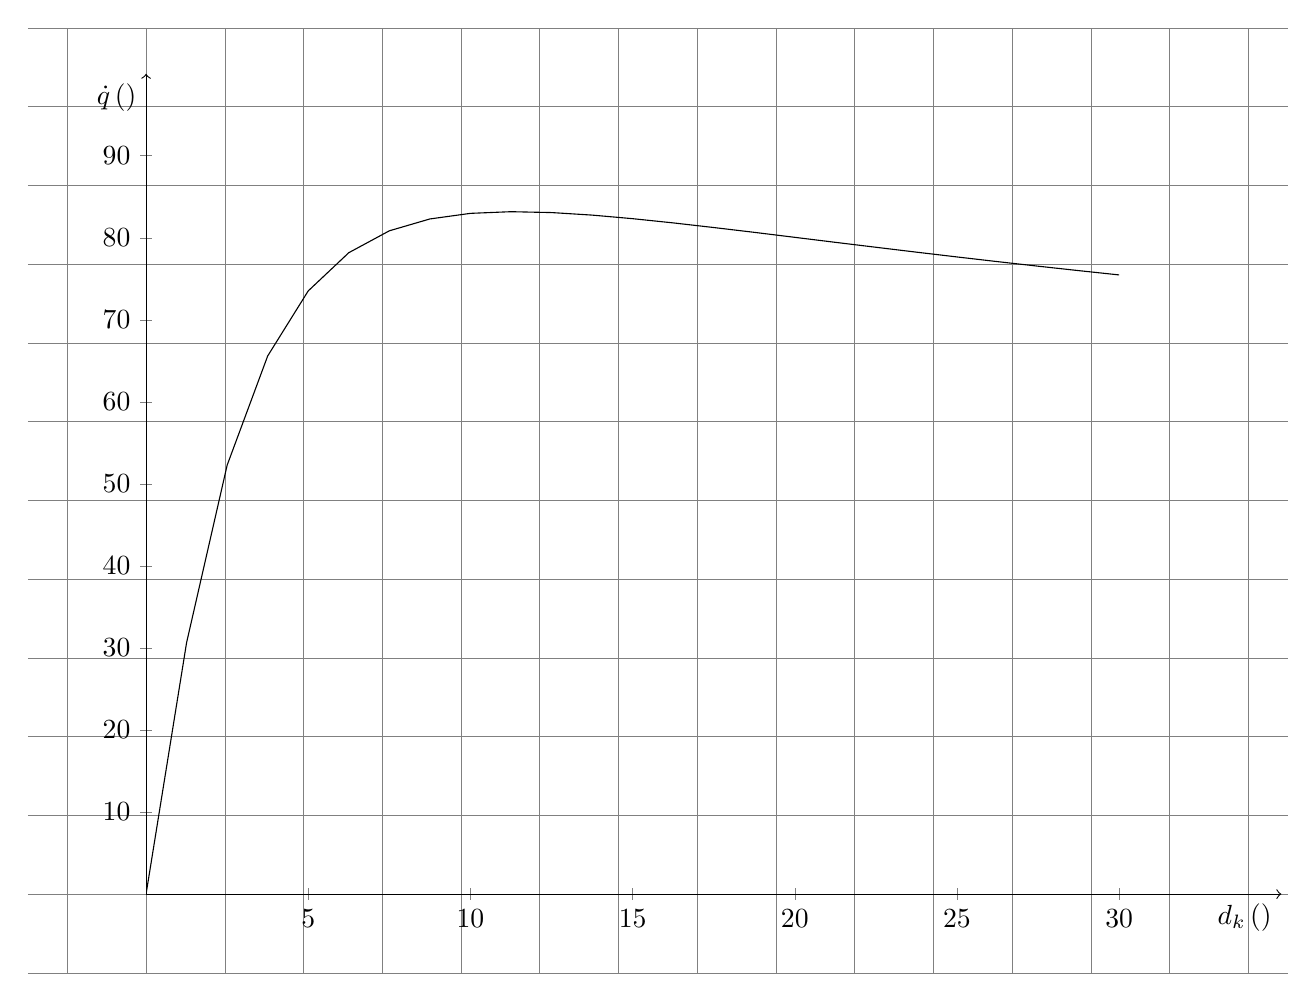
\begin{tikzpicture}
	% Rács és vágómaszk
	\draw[step=1cm, gray, very thin] (-1.5, -1) grid (14.5, 11);
	%\clip (-1.5, -1) rectangle (14.5, 11);
	
	% A tengelykeresztet az axis környezet hozza létre
			\begin{axis}[
	width=16cm, height=12cm,
	xmin=0, xmax=35,
	ymin=0, ymax=100, 
	axis lines = middle,
	axis line style={->},
	xlabel=$d_{k} \left(\si{\meter}\right)$, 
	xlabel style={
		at=(current axis.right of origin), 
		anchor=north east
	}, 
	ylabel=$\dot{q} \left(\si{\watt\per\meter\squared}\right)$, 
	ylabel style={
		at=(current axis.above origin), 
		anchor=north east
	},
	xtick={5, 10, 15, 20, 25, 30},
	ytick={10, 20, 30, 40, 50, 60, 70, 80, 90}
	]
	

		\addplot [black, domain=0:30] {1/(ln(x/1)/(2*3.1416*45.4)+1/(8*x*3.1416))};
		
		
	\end{axis}
	
	\end{tikzpicture}
	\caption{Hőáram-átmérő diagram acélcső esetén}
\end{figure}

\begin{figure}[h]
	\centering
	\label{figure:guh7ud-vgpvd}
	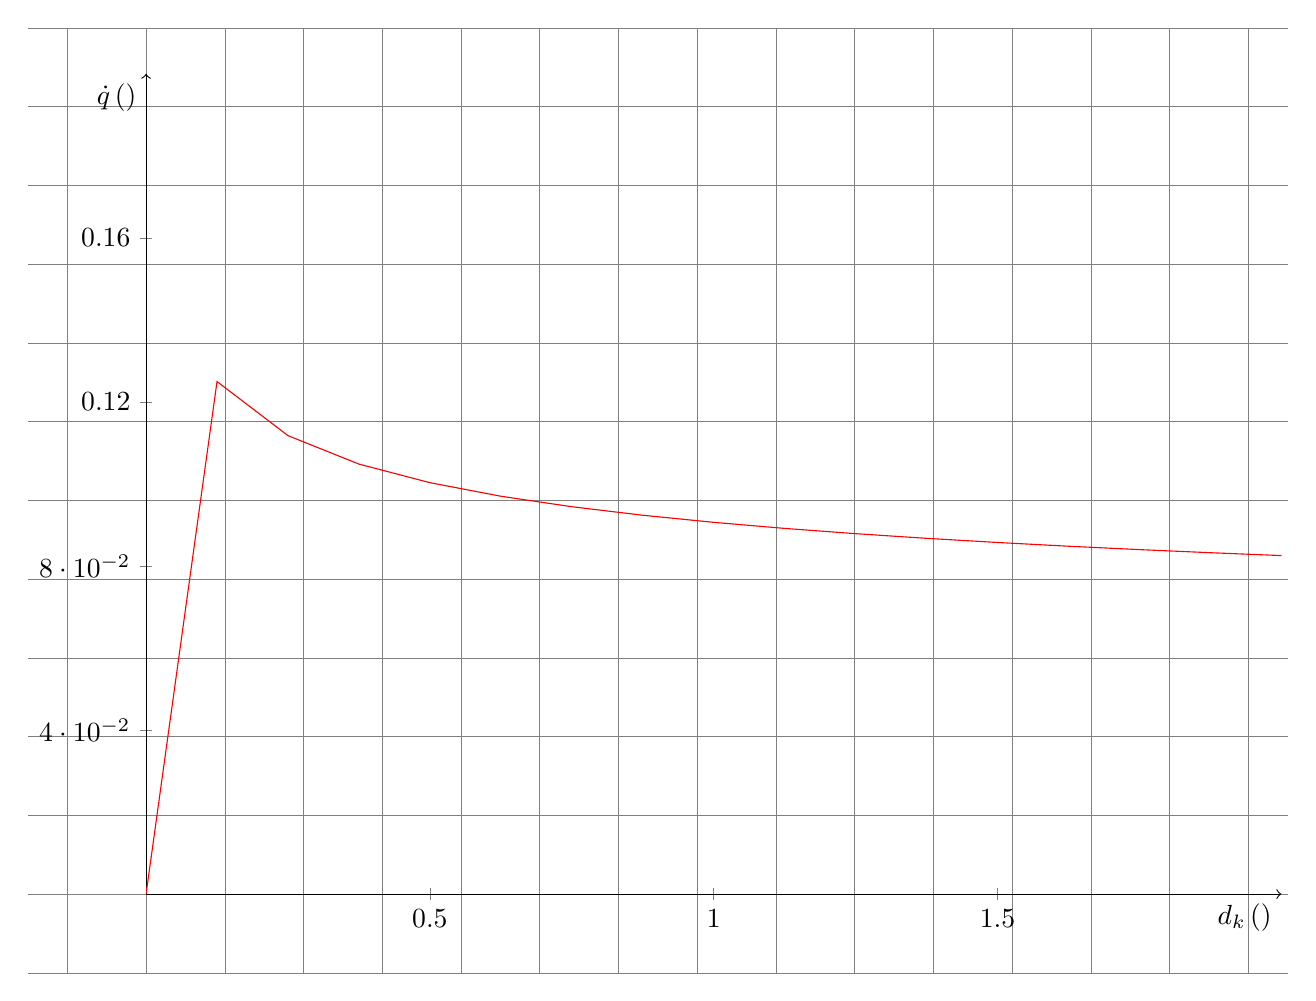
\begin{tikzpicture}
	% Rács és vágómaszk
	\draw[step=1cm, gray, very thin] (-1.5, -1) grid (14.5, 11);
	%\clip (-1.5, -1) rectangle (14.5, 11);
	
	% A tengelykeresztet az axis környezet hozza létre
	\begin{axis}[
	width=16cm, height=12cm,
	xmin=0, xmax=2,
	ymin=0, ymax=0.2, 
	axis lines = middle,
	axis line style={->},
	xlabel=$d_{k} \left(\si{\meter}\right)$, 
	xlabel style={
		at=(current axis.right of origin), 
		anchor=north east
	}, 
	ylabel=$\dot{q} \left(\si{\watt\per\meter\squared}\right)$, 
	ylabel style={
		at=(current axis.above origin), 
		anchor=north east
	},
	xtick={0.5, 1, 1.5},
	ytick={0.04, 0.08, 0.12, 0.16}
	]
	
	
	\addplot [red, domain=0:3] {1/(ln(x/0.001)/(2*3.1416*0.1)+1/(8*x*3.1416))};
	
	\end{axis}
	
	\end{tikzpicture}
	\caption{Hőáram-átmérő diagram azbeszt-cementcső esetén}
\end{figure}


% Oldaltörés
\pagebreak